\documentclass[a4paper]{amsart}
\usepackage[utf8]{inputenc}
\usepackage{lmodern}
\usepackage{microtype}

\usepackage{commath}

\usepackage{tikz}
\usepackage{graphicx}
\usepackage{siunitx}

\usepackage[hidelinks]{hyperref}
\usepackage[noabbrev]{cleveref}

\def\signed #1{{\leavevmode\unskip\nobreak\hfil\penalty50\hskip2em
  \hbox{}\nobreak\hfil(#1)%
  \parfillskip=0pt \finalhyphendemerits=0 \endgraf}}
\newsavebox\mybox
\newenvironment{aquote}[1]
  {\savebox\mybox{#1}\begin{quote}}
  {\signed{\usebox\mybox}\end{quote}}

\newcommand{\df}[1]{\textbf{#1}}

\swapnumbers
\newtheorem{thm}{Theorem}[section]
\newtheorem{lem}[thm]{Lemma}
\theoremstyle{definition}
\newtheorem{defn}[thm]{Definition}
\newtheorem{ex}[thm]{Example}
\newtheorem{exercise}[thm]{Exercise}
\theoremstyle{remark}
\newtheorem{rem}[thm]{Remark}

\title[Level 1 Mathematics: Algebra and Patterns]{Level 1 Algebra (91027)\\Level 1 TEG (91028)}
\author{Alexander Elzenaar}
\date{\today}

\begin{document}
  \maketitle
  \section{What is Algebra?}
  \begin{aquote}{Ian Stewart --- \textit{Taming the Infinite}}
    At school level, algebra is a branch of mathematics in which unknown numbers are represented by letters, the operations
    of arithmetic are represented by symbols, and the main task is to deduce the values of unknown quantities from equations...
    In advanced mathematics, the use of symbols to represent numbers is only one tiny aspect of the subject, the context in which
    it got started. Algebra is about the properties of symbolic expressions in their own right; it is about structure and form,
    not just number.
  \end{aquote}

  \begin{aquote}{Artin --- \textit{Algebra}}
    \noindent``One, two, three, five, four...''

    \noindent``No Daddy, it's one, two, three, four five.''

    \noindent``Well if I want to say one, two, three, five, four, why can't I?''

    \noindent``That's not how it goes.''
  \end{aquote}

  \begin{figure}
    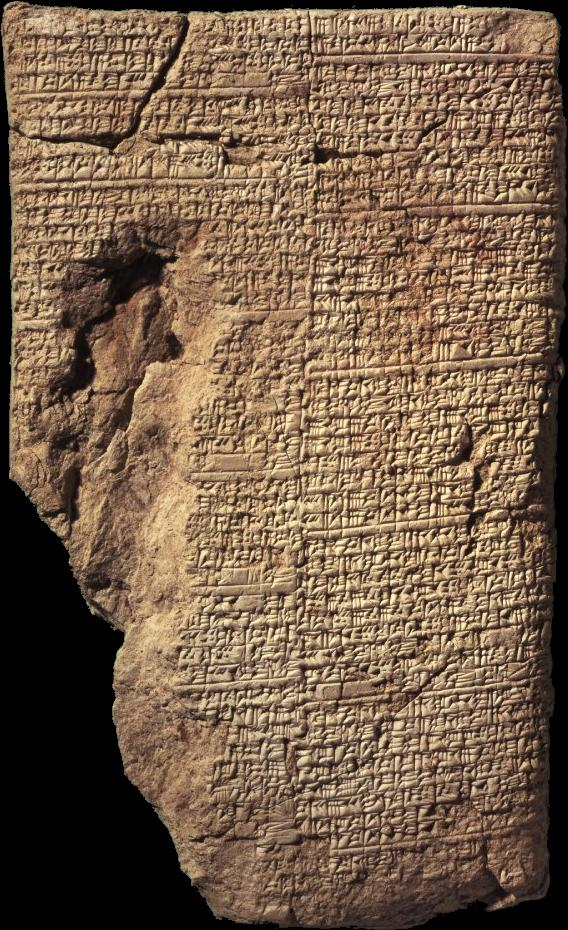
\includegraphics[width=0.3\textwidth]{babylon-small}
    \caption{A Babylonian tablet with a quadratic equation.\label{fig:babylon}}
  \end{figure}

  High-school algebra (the finding solutions for unknown quantities from given values) is an ancient subject; the ancient Babylonians
  were solving some form of complex equations around 4000 years ago, and clay tablets dating from around 1700 BCE show evidence of
  algebraic methods (see \cref{fig:babylon}).

  What can we do with numbers?
  \begin{itemize}
    \item Add and subtract ($ 3 + 4 = 7 $)
    \item Multiply and divide ($ 2 \times 8 = 16 $)
    \item Take powers and roots ($ 3^3 = 27 $)
    \item Apply functions ($ \sin (\ang{90}) = 1 $)
  \end{itemize}
  \begin{ex}
    With numbers, we can solve a number of practical problems.
    \begin{itemize}
      \item How many sheep do I own?
      \item If I eat three sheep, how many sheep do I have now?
      \item Do I have more sheep than Alan?
      \item If I steal Alan's sheep, how many will I have?
    \end{itemize}
  \end{ex}

  Very useful, but we need something more abstract in order to solve more complicated practical problems.
  \begin{ex}\label{ex:manybirds}
    A man buys thirty birds --- partridges, doves, and sparrows. A partridge costs three silver coins,
    a dove two, and a sparrow $1/2$. He pays thirty silver coins. How many birds of three kinds does he buy?
  \end{ex}
  We could solve this without algebra, but it would be confusing and longwinded.

  If we rewrite \cref{ex:manybirds} but this time in a more formal symbolism (calling the number of partridges, doves, and sparrows $ s $, $ d $,
  and $ p $ respectively), it looks like:
  \begin{equation}
    \begin{cases}
      p + d + s = 30\\
      3p + 2d + \frac{1}{2}s = 30.
    \end{cases}
  \end{equation}
  This form of the problem looks harder to understand, but it is much easier to find a solution for it \emph{because
  now it looks exactly the same as every other problem}. We have abstracted away the details (what things we're dealing
  with) and are left with the minimal amount of information needed to solve the problem!

  \section{Topics for Algebra}
  (Unless otherwise stated, references are to \textit{Theory and Problems of College Algebra} by Murray Spiegel [512 S75].)
  \subsection{Polynomials and Simplification}
  \begin{itemize}
    \item Definition of polynomial.
    \item Reading: ch. 2, pp.11-4.
    \item Problems: pp.19-20, qns 10,12-6.
  \end{itemize}
  \subsection{Factorisation}
  Recall that most integers can be written as the product of (at least) two SMALLER integers: e.g. $ 14 = 7 \times 2 $. The same
  is true for polynomials. For example, $ 7x + 3x^2 = x(7 + 3x) $. This is just a small glimpse at the comparison between integers
  and polynomials; both form what is known as a \df{ring}.

  Note that $ (x + a)(x + b) = x^2 + (a + b)x + ab $. In other words, we can factorise quadratics if we can find two numbers $ a $ and $ b $
  which sum to the coefficient of the $ x $ term and multiply to the constant term. If there is some coefficient on the $x^2 $ term, there is
  also an algorithm which can be used but it is a little more complicated.
  \begin{itemize}
    \item Reading: see above.
    \item Problems: pp.33-4, qns 13-8.
  \end{itemize}

  \subsection{Rational Expressions}
  \begin{itemize}
    \item Reading: ch. 5, p.35 ONLY.
    \item Problems: pp.40-1, qns. 6-11.
  \end{itemize}

  \subsection{Exponents}
  \begin{itemize}
    \item Reading: ch. 6, pp. 42-3.
    \item Problems: pp.51-2, qns. 19,20,22.
  \end{itemize}

  \subsection{Functions and Graphs}
  \begin{itemize}
    \item Reading: ch. 10, pp. 75-7.
    \item Problems: pp.85-6, qns. 23, 24, 25, 27, 38, 43, 44-6.
  \end{itemize}

  \subsection{Linear Equations}
  \begin{itemize}
    \item Problems: pp. 95-8, all probs
  \end{itemize}

  \subsection{Quadratic Equations (examinable by inspection ONLY)}
  \begin{itemize}
    \item Reading: ch. 13, pp.110-1 (incl. quad formula)
    \item Problems: pp.123-5, qns 31, 34, 35, 37, 38, 42-4.
  \end{itemize}

  \subsection{Quadratic Patterns and Graphs}
  \begin{itemize}
    \item Reading: proof that 2nd difference is leading coefficient if step is 1.
    \item Problems: StudyPass revision guide pp.34-40.
  \end{itemize}

  \subsection{Inequations}
  \begin{itemize}
    \item Reading: ch. 19, pp.167-8.
    \item Problems: pp. 171, all probs
  \end{itemize}

  \subsection{Exponential Equations}
  \begin{itemize}
    \item Reading: TBD.
    \item Problems: TBD.
  \end{itemize}

  \subsection{Optimisation Without Calculus}
  \begin{itemize}
    \item \textit{Maxima and minima without calculus} by Ivan Niven [515.64 N73].
    \item StudyPass revision guide p.47.
  \end{itemize}

  \subsection{Systems of Linear Eqns}
  \begin{itemize}
    \item Reading: ch. 12, pp.100-1
    \item Problems: pp.107-9, qns. 26-7, 29, 30-4, 37-8.
  \end{itemize}

  \subsection{Consolidation}
  \begin{itemize}
    \item Past papers.
  \end{itemize}

  \section{Fun Stuff}
  This year, the focus is on learning the techniques and ideas that will be used in higher mathematics rather than on doing
  any mathematics for its own sake --- think of it as learning the grammar of a new language, rather than actually speaking
  or reading that language. This is why the material is best learned as rote after you understand the ideas behind it: like
  the mutiplication table, you should know this material within your soul before you start doing any actual mathematics next
  year!

  Because I understand how boring it is to learn this material without any interesting interludes, I like to (at Y11 and Y12)
  run each hourly session as follows:
  \begin{itemize}
    \item 45 min. of `grammar' (e.g. `linear equations' in this case)
    \item 15 min. of real mathematics (NON-EXAMINABLE interesting material)
  \end{itemize}
  The following is an indicative list of topics that fall into the latter category that I am happy to talk about to Y11/12
  students. The aim is to give students an idea of what `real mathematicians' actually do or study, but not to actually teach
  the details; think of it like an overview of a bunch of interesting topics. YOU DO NOT NEED TO LEARN OR STUDY THIS MATERIAL!
  You only need to be interested (and I guarantee that this material is interesting). THIS MATERIAL IS NOT TESTED (at college, anyway).

  \begin{itemize}
    \item Sets and infinity (Russell's paradox, cardinality)
    \item Development of the number system (Peano's axioms, following Landau)
    \item Number theory (various topics)
    \item Logic and G\"odel's theorem (is arithmetic consistent?)
    \item Greek mathematics
    \item Fibonnacci
    \item Euclidean geometry
    \item Conic sections
    \item Geometries other than Euclid's
    \item Projective geometry
    \item Topology and knots
    \item Galois and the constructability of geometric figures (sad man with big plans)
    \item Fermat's Last Theorem (the biggest media event in mathematics of the 20th century?)
    \item Graph theory (4-colour theorem)
    \item How to count (combinatorics)
    \item Linear algebra (geometric)
    \item Group theory and symmetry
    \item Rings (the link between numbers, polynomials, continuous functions)
    \item Complex numbers (natural numbers $\rightarrow$ integers $\rightarrow$ rational numbers $\rightarrow$ real numbers $\rightarrow$ ???)
    \item Calculus (the mathematics of change)
    \item Cryptography
    \item Probability
    \item The mathematics of population
    \item Some random physics(?)
  \end{itemize}

  \clearpage
  \section{Assorted Proofs}
  The following are a set of proofs for my own reference.
  \begin{defn}
    Let $ f $ be some function from and to the reals. Then for every $ \varepsilon > 0 $ the \df{finite $ \varepsilon-$difference} of $ f $
    at $ x $ is $ f_{-\varepsilon} = f(x + \varepsilon) - f(x) $. The second finite $\varepsilon$-difference at $ x $
    is $ f_{-\varepsilon^2} = \left(f_{-\varepsilon}\right)_{-\varepsilon} $, and the $ n$th finite $ \varepsilon$-difference is defined
    recursively in the obvious way.
  \end{defn}
  \begin{thm}[quadratic means constant second finite difference]
    Suppose we have some continuous function $ f : \mathbb{R} \to \mathbb{R} $, such that $ f(x) = y_0 $, $ f(x + \varepsilon) = y_1 $,
    and $ f(x + 2\varepsilon) = y_2 $. If $ f $ is a quadratic polynomial, then $ f_{-\varepsilon^2} $ is constant for any given $\varepsilon$
    and $ f $ has leading coefficient $ \frac{f_{-\varepsilon^2}}{2\epsilon^2} $.
  \end{thm}
  \begin{proof}
    Suppose $ f(x) = ax^2 + bx + c $. Then:
    \begin{align*}
      f_{-\varepsilon^2} &= y_2 - 2y_1 + y_0\\
                         &= a(x + 2\varepsilon)^2 + b(x + 2\varepsilon) + c - 2a(x + \varepsilon)^2 - 2b(x + \varepsilon) - 2c + ax^2 + bx + c\\
                         &= 2a\varepsilon^2.
    \end{align*}
    The theorem follows.
  \end{proof}
  Hence we can find the leading term given a nice table.

  \begin{thm}[constant second finite derivative means quadratic]
    If $ f $ is continuous on $ \mathbb{R} $ and for every $\varepsilon$ $ f_{-\varepsilon^2}(x) = \lambda(x) $ is constant, then $ f $ is a polynomial
    of degree at most 2 (i.e. at worst, $ f $ is quadratic).
  \end{thm}
  \begin{proof}
    Let $ g = f_{-\varepsilon} $. Note that $ \frac{g_{-\varepsilon}}{\varepsilon} = \frac{g(x + \varepsilon) - g(x)}{\varepsilon} = \frac{\lambda(x)}{\varepsilon} $.
    Take $ \varepsilon \to 0 $;  then we have $ g'(x) = \lim_{\varepsilon \to 0} \frac{\lambda(x)}{\varepsilon} $. Play the same game again and we find that
    \begin{displaymath}
      f''(x) = \lim_{\varepsilon \to 0} \frac{\lambda(x)}{\varepsilon^2}.
    \end{displaymath}
    In particular, $ f''(x) $ is either constant or blows up to infinity everywhere (depending on `how dependent' $\lambda$ is on $\varepsilon$). But $ f $ is
    continuous everywhere, so $ f''(x) < \infty $. Hence $ f''(x) = 2a $ for some $ a \in \mathbb{R} $, and $ f(x) = ax^2 + bx + c $.
  \end{proof}

\clearpage
\section{Interest Topic: Sets and Infinity}
\begin{aquote}{Halmos}
  A pack of wolves, a bunch of grapes, or a flock of pigeons are all examples of sets of things. The mathematical concept of a set can
  be used as the foundation for all known mathematics...
\end{aquote}
\begin{ex}Some examples of sets:-
  \begin{enumerate}
    \item The set of all people (finite).
    \item The set of all natural numbers, $ \mathbb{N} = \{1,2,3,\dots\} $ (infinite).
    \item The set of all real numbers, $ \mathbb{R} $ (finite).
    \item The set $ S = \{1,2,3\} $ (finite).
    \item The set $ R = \{a, b, c\} $ (finite).
  \end{enumerate}
\end{ex}

Clearly $ S $ and $ R $ are the `same size'. But what does `size' mean?

Bijection: to every element of $ S $ we can assign exactly one element of $ R $ such that there are none left over. So
we can tell if two sets are the same size without needing any notion of `counting'.

We define $ 0 = \{\} $, $ 1 = \{0\} $, $ 2 = \{0, 1\} $, $ 3 = \{0,1,2\} $ and so on. A set is called finite if it is the
same size as some natural number, otherwise it is called infinite.

If a set is infinite, then it has a subset of the same size. (For example, $ 2\mathbb{N} $ in $ \mathbb{N} $.)

Are there different sizes of infinity? Natural numbers and rational numbers are the same size. But real numbers?

For any potential pairing of real numbers with natural numbers, I can write down a number not on the list. Hence there
can be no such pairing (there will always be real numbers not left over) and hence there are \emph{more} real numbers
than natural numbers (even though both are finite).

There are sets even bigger than the real numbers.

How big can we make sets? Can we have a set of all sets? No. For consider the set $ B $ that contains all sets in some bigger set $ A $ which do not
contain themselves. Can $ B $ be in $ A $? No --- for if $ B $ were in $ A $, then either $ B $ is in $ B $ or $ B $ is not in $ B $. If it is, then it does
not contain itself --- but it does! If it is not, then it does contain itself --- but it doesn't! Hence there is at least one set $ B $ that is not in $ A $
\emph{for any set $ A $} --- so no set is big enough to contain all other sets (Russell's paradox).

In other words, \emph{nothing contains everything}: that is, \emph{there is no universe} (universe of discourse, that is: a set of all possible things
that enter into a discussion).

\end{document}
